% Topic from _Linear Algebra_ Jim Hefferon
%  http://joshua.smcvt.edu/linalg.html
%  2012-Feb-12
\topic{Magic Squares}
\index{magic squares|(}
According to legend, 
in ancient China there was a flood in the Lo river.
The people offered sacrifices to the river, 
to appease him.
Each time from the river emerged a turtle, one of the celestial animals, 
and walked around the sacrifice.
Fuh-Hi (2858-2738~BC), the founder of Chinese civilization,  
interpreted this to say that
the river had not accepted the sacrifice.  
Then a child noticed that the turtle had on its shell what is today
known as the Lo Shu pattern.
\begin{center}
  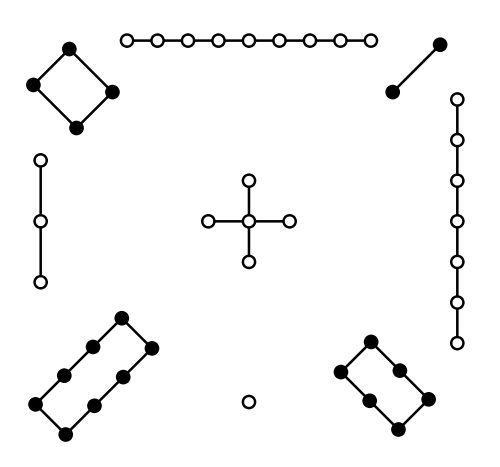
\includegraphics{LoShu.png}
\end{center}
Counting the dots gives a matrix.
\begin{center}
  \begin{tabular}{|c|c|c|}
    \hline
      $4$  &$9$  &$2$  \\ \hline
      $3$  &$5$  &$7$  \\ \hline
      $8$  &$1$  &$6$  \\ \hline    
  \end{tabular}
\end{center}
Each row, column, 
and diagonal adds to $15$
(the number of days in each of the twenty four cycles of the Chinese solar year).
Now that the people knew how much to sacrifice, they at last appeased the river.
(http://en.wikipedia.org/wiki/Lo_Shu_Square)

\textit{Melencolia I} is an engraving by Albrecht D\"urer.
(http://en.wikipedia.org/wiki/Melencolia_I)
\begin{center}
  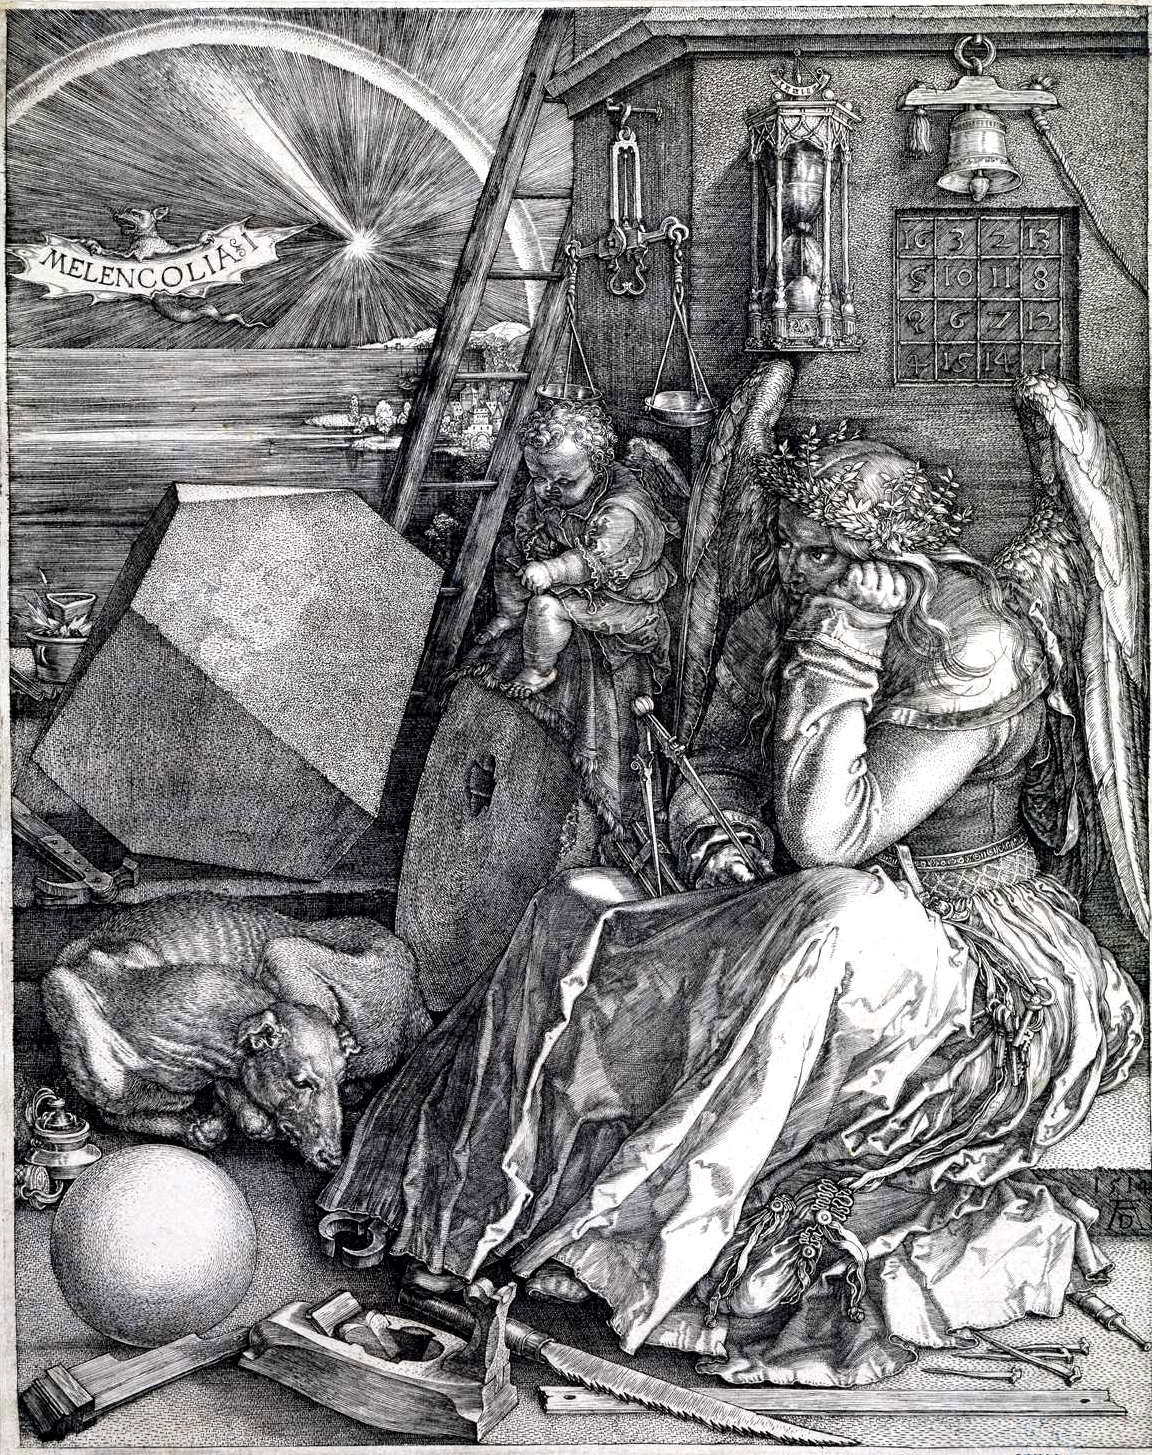
\includegraphics{Melencolia.jpg} % wikipedia http://upload.wikimedia.org/wikipedia/commons/1/14/Melencolia_I_%28Durero%29.jpg
\end{center}
One interpretation is that it depicts the melancholy or depressive state.
The figure, representing genius,
is surrounded by a wealth of fascinating things to be discovered an explored, 
including
the compass, the geometrical solid, the scale, and the hourglass.
But the figure seems unmoved; all the things are unused.
One of the potential delights is the $\nbyn{4}$ matrix in the upper right.
The rows, columns, and diagonals add to $34$.
\begin{center}
  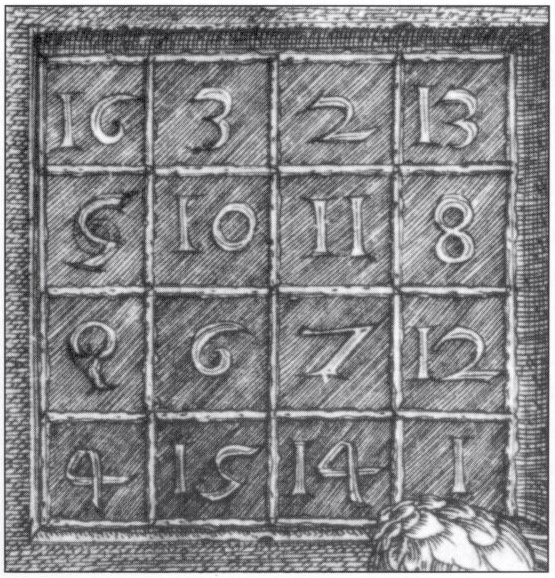
\includegraphics{Melencoliadetail.jpg} % wikipedia http://upload.wikimedia.org/wikipedia/commons/7/7e/Albrecht_D%C3%BCrer_-_Melencolia_I_%28detail%29.jpg
\end{center}
The middle entries on the bottom row give $1514$, the 
date of the engraving.

A \definend{magic square}\index{magic square}\index{matrix!magic square}
is a square matrix such that each row, column, and diagonal add to the same
value.

Every $\nbyn{1}$ square is magic.
For the $\nbyn{2}$ case, if the rows, columns, and diagonals add to $k$
\begin{equation*}
  \begin{mat}
    a  &b  \\
    c  &d
  \end{mat}
\end{equation*}
then $a+b=k$, $c+d=k$, $a+c=k$, $b+d=k$, $a+d=k$, and $b+c=k$.
Taking only the first four of those, the associated homogeneous system
\begin{equation*}
  \begin{amat}{4}
        
  \end{amat}
\end{equation*}




It is an unsolved problem to determine the number of magic squares of an arbitrary order, but the number of distinct magic squares (excluding those obtained by rotation and reflection) of order n=1, 2, ... are 1, 0, 1, 880, 275305224, ... (Sloane's A006052; Madachy 1979, p. 87). The 880 squares of order four were enumerated by Frénicle de Bessy in 1693, and are illustrated in Berlekamp et al. (1982, pp. 778-783). The number of 5×5 magic squares was computed by R. Schroeppel in 1973. The number of 6×6 squares is not known, but Pinn and Wieczerkowski (1998) estimated it to be (1.7745+/-0.0016)×10^(19) using Monte Carlo simulation and methods from statistical mechanics. 
(http://mathworld.wolfram.com/MagicSquare.html)
\begin{equation*}
  \begin{linsys}{7}
    i_0  &-  &i_1  &-  &i_2  &   &    &  &    &   &    &  &    &=  &0  \\
         &   &i_1  &   &     &-  &i_3 &  &    &-  &i_5 &  &    &=  &0  \\
         &   &     &   &i_2  &   &    &- &i_4 &+  &i_5 &  &    &=  &0  \\
         &   &     &   &     &   &i_3 &+ &i_4 &   &    &- &i_6 &=  &0  \\
         &   &5i_1 &   &     &+  &10i_3  &  & &   &    &  &    &=  &10  \\
         &   &     &   &2i_2 &   &    &+ &4i_4 &  &    &  &    &=  &10  \\
         &   &5i_1 &-  &2i_2 &   &    &  &    &+  &50i_5 &&    &=  &0   
  \end{linsys}
\end{equation*}
It can be done by hand, but it would take a while and be error-prone.
Using a computer is better.

We illustrate by solving that system under Sage.
\begin{lstlisting}
sage: var('i0,i1,i2,i3,i4,i5,i6')
(i0, i1, i2, i3, i4, i5, i6)
sage: network_system=[i0-i1-i2==0, i1-i3-i5==0, 
....:       i2-i4+i5==0,, i3+i4-i6==0, 5*i1+10*i3==10,
....:       2*i2+4*i4==10, 5*i1-2*i2+50*i5==0]
sage: solve(network_system, i0,i1,i2,i3,i4,i5,i6)     
[[i0 == (7/3), i1 == (2/3), i2 == (5/3), i3 == (2/3), 
      i4 == (5/3), i5 == 0, i6 == (7/3)]] 
\end{lstlisting}
Magic.

Here is the same system solved under Maple.
We enter the array of coefficients 
and the vector of constants,
and then we get the solution.
\begin{lstlisting}
> A:=array( [[1,-1,-1,0,0,0,0],
             [0,1,0,-1,0,-1,0],
             [0,0,1,0,-1,1,0],
             [0,0,0,1,1,0,-1],
             [0,5,0,10,0,0,0],
             [0,0,2,0,4,0,0],
             [0,5,-2,0,0,50,0]] );
> u:=array( [0,0,0,0,10,10,0] );
> linsolve(A,u);
      7  2  5  2  5     7
    [ -, -, -, -, -, 0, - ]
      3  3  3  3  3     3
\end{lstlisting}

Systems with infinitely many solutions are entered in the same
way but for the solution the computer will return a parametrization.




\begin{exercises}
  % \item[]\textit{Answers for this Topic use Maple as
  %                               the computer algebra system.
  %                               In particular, all of these were tested
  %                               on Maple~$V$ running under MS-DOS
  %                               NT version~$4.0$.
  %                               (On all of them, the preliminary command
  %                               to load the linear algebra package
  %                               %\protect\mbox{\texttt{with(linalg);}},
  %                               along with Maple's responses to the 
  %                               Enter key, 
  %                               have been omitted.)
  %                               Other systems have similar
  %                               commands.}
  \item 
    Use the computer to solve the two problems that opened this
    chapter.
    \begin{exparts}
      \partsitem This is the Statics problem.
         \begin{align*}
            40h+15c  &= 100  \\
            25c      &= 50+50h
         \end{align*}
      \partsitem This is the Chemistry problem.
         \begin{align*} 
             7h      &= 7j  \\
             8h +1i  &= 5j+2k  \\
             1i      &= 3j  \\
             3i      &= 6j+1k
         \end{align*}
    \end{exparts}
    \begin{answer}
      \begin{exparts}
        \partsitem The commands
\begin{indented}{\small
\begin{verbatim}
> A:=array( [[40,15],
             [-50,25]] );
> u:=array([100,50]);
> linsolve(A,u);
\end{verbatim}
}\end{indented}
           yield the answer $[1,4]$.
        \partsitem Here there is a free variable:
\begin{indented}{\small
\begin{verbatim}
> A:=array( [[7,0,-7,0],
             [8,1,-5,2],
             [0,1,-3,0],
             [0,3,-6,-1]] );
> u:=array([0,0,0,0]);
> linsolve(A,u);
\end{verbatim}
}\end{indented}
         prompts the reply $[\_t_1,3\_t_1,\_t_1,3\_t_1]$.
      \end{exparts}
    \end{answer}
\item 
    Use the computer to solve these systems from the
    first subsection,
    or conclude `many solutions' or `no solutions'.
    \begin{exparts*}
      \partsitem \(
               \begin{linsys}[t]{2}
                  2x  &+  &2y  &=  &5  \\
                   x  &-  &4y  &=  &0  
               \end{linsys}
             \)
      \partsitem \(
               \begin{linsys}[t]{2}
                  -x  &+  &y   &=  &1  \\
                   x  &+  &y   &=  &2  
               \end{linsys}
             \) 
      \partsitem  \(
               \begin{linsys}[t]{3}
                   x  &-  &3y  &+  &z  &=  &1  \\
                   x  &+  &y   &+  &2z &=  &14 
                \end{linsys}
             \) 
      \partsitem  \(
               \begin{linsys}[t]{2}
                  -x  &-  &y   &=  &1  \\
                 -3x  &-  &3y  &=  &2  
               \end{linsys}
             \) 
      \partsitem  \(
               \begin{linsys}[t]{3}
                      &   &4y  &+  &z  &=  &20 \\
                  2x  &-  &2y  &+  &z  &=  &0  \\
                   x  &   &    &+  &z  &=  &5  \\
                   x  &+  &y   &-  &z  &=  &10 
                \end{linsys}
             \)
      \partsitem \( \begin{linsys}[t]{4}
                 2x  &   &   &+  &z  &+  &w  &=  &5  \\
                     &   &y  &   &   &-  &w  &=  &-1 \\
                 3x  &   &   &-  &z  &-  &w  &=  &0  \\
                 4x  &+  &y  &+  &2z &+  &w  &=  &9  
               \end{linsys}
            \)
    \end{exparts*}
    \begin{answer}
      These are easy to type in.
      For instance, the first  
\begin{indented}{\small
\begin{verbatim}
> A:=array( [[2,2],
             [1,-4]] );
> u:=array([5,0]);
> linsolve(A,u);
\end{verbatim}
}\end{indented}
      gives the expected answer of $[2,1/2]$.
      The others are entered similarly.
      \begin{exparts}
        \partsitem The answer is \( x=2 \) and \( y=1/2 \).
        \partsitem The answer is \( x=1/2 \) and \( y=3/2 \). 
        \partsitem This system has infinitely many solutions.
           In the first subsection, with $z$ as a parameter, 
           we got $x=(43-7z)/4$ and $y=(13-z)/4$.
           Maple responds with $[-12+7\_t_1,\_t_1,13-4\_t_1]$,
           for some reason preferring $y$ as a parameter.
        \partsitem There is no solution to this system.
           When the array $A$ and vector $u$ are given to Maple
           and it is asked to \texttt{linsolve(A,u)}, 
           it returns no result at all, that is, it responds with
           no solutions.
        \partsitem The solutions is \( (x,y,z)=(5,5,0) \).
        \partsitem There are many solutions.
           Maple gives $[1,-1+\_t_1,3-\_t_1,\_t_1]$.
      \end{exparts}
    \end{answer}
  \item 
    Use the computer to solve these systems from the second subsection.
    \begin{exparts*}
      \partsitem \( \begin{linsys}[t]{2}
                  3x  &+  &6y  &=  &18  \\
                   x  &+  &2y  &=  &6   
                   \end{linsys}  \)
      \partsitem \( \begin{linsys}[t]{2}
                   x  &+  &y   &=  &1  \\
                   x  &-  &y   &=  &-1   
                    \end{linsys}  \)
      \partsitem \( \begin{linsys}[t]{3}
                   x_1  &   &     &+  &x_3   &=  &4  \\
                   x_1  &-  &x_2  &+  &2x_3  &=  &5  \\
                  4x_1  &-  &x_2  &+  &5x_3  &=  &17  
                   \end{linsys}  \)
      \partsitem \( \begin{linsys}[t]{3}
                   2a   &+  &b    &-  &c     &=  &2  \\
                   2a   &   &     &+  &c     &=  &3  \\
                    a   &-  &b    &   &      &=  &0   
                    \end{linsys}  \)
      \partsitem \( \begin{linsys}[t]{4}
                     x  &+  &2y   &-   &z   &    &    &=  &3  \\
                    2x  &+  &y    &    &    &+   &w   &=  &4  \\
                     x  &-  &y    &+   &z   &+   &w   &=  &1  
                    \end{linsys}  \)
      \partsitem \( \begin{linsys}[t]{4}
                     x  &   &     &+   &z   &+   &w   &=  &4  \\
                    2x  &+  &y    &    &    &-   &w   &=  &2  \\
                    3x  &+  &y    &+   &z   &    &    &=  &7  
                     \end{linsys}  \)
    \end{exparts*}
    \begin{answer}
      As with the prior question, entering these is easy.
      \begin{exparts}
        \partsitem This system has infinitely many solutions. 
              In the second subsection we gave the solution set as
              \begin{equation*}
              \set{\colvec{6 \\ 0}+\colvec{-2 \\ 1}y
                      \suchthat y\in\Re}
              \end{equation*}
              and Maple responds with $[6-2\_t_1,\_t_1]$.
        \partsitem The solution set has only one member
          \begin{equation*}
             \set{\colvec{0 \\ 1} }
          \end{equation*}
          and Maple has no trouble finding it $[0,1]$.
        \partsitem This system's solution set is infinite
          \begin{equation*}
            \set{\colvec{4 \\ -1 \\ 0}+\colvec{-1 \\ 1 \\ 1}x_3
                             \suchthat x_3\in\Re}
          \end{equation*}
          and Maple gives $[\_t_1,-\_t_1+3,-\_t_1+4]$.
        \partsitem There is a unique solution
           \begin{equation*}
             \set{\colvec{1 \\ 1 \\ 1}}
           \end{equation*}
           and Maple gives $[1,1,1]$.
        \partsitem This system has infinitely many solutions; in the 
           second subsection we described the solution set with
           two parameters
           \begin{equation*}
             \set{\colvec{5/3 \\ 2/3 \\ 0 \\ 0}
                  +\colvec{-1/3 \\ 2/3 \\ 1 \\ 0}z
                  +\colvec{-2/3 \\ 1/3 \\ 0 \\ 1}w
                  \suchthat z,w\in\Re}
           \end{equation*}
           as does Maple $[3-2\_t_1+\_t_2,\_t_1,\_t_2,-2+3\_t_1-2\_t_2]$.
        \partsitem The solution set is empty and Maple replies to the
           \texttt{linsolve(A,u)} command with no returned solutions.
      \end{exparts}
    \end{answer}
  \item 
    What does the computer give for the solution of the general
    $\nbyn{2}$  system?
    \begin{equation*}
      \begin{linsys}{2}
        ax  &+  &cy  &=  &p  \\
        bx  &+  &dy  &=  &q
      \end{linsys}
    \end{equation*}
    \begin{answer}
       In response to this prompting
\begin{indented}{\small
\begin{verbatim}
> A:=array( [[a,c],
             [b,d]] );
> u:=array([p,q]);
> linsolve(A,u);
\end{verbatim}
}\end{indented}
      Maple thought for perhaps twenty seconds and gave this reply.
      \begin{equation*}
        \bigl[-\frac{-d\,p+q\,c}{-b\,c+a\,d},
          \frac{-b\,p+a\,q}{-b\,c+a\,d}\bigr]
      \end{equation*}
    \end{answer}
\end{exercises}
\index{magic squares|)}
\endinput


